\documentclass{article}

\usepackage{url} 
\usepackage{geometry,afterpage}
\usepackage{pdfpages}
\usepackage{lastpage}
\usepackage{fancyhdr}
\usepackage{ngerman}
\usepackage{listings}

\usepackage{floatrow}
\usepackage[tableposition=top]{caption}
\floatsetup[table]{capposition=top}

\usepackage{amsmath, amssymb}

\usepackage[utf8]{inputenc}


\usepackage[numbib]{tocbibind}



\newcommand\twodigits[1]{%
   \ifnum#1<10 0#1\else #1\fi
}



\lhead{Röntgenfluoreszenzanalyse}
\rhead{04.06.2021\\ J. Winkler}
%\cfoot{\twodigits{\thepage}~/ \pageref{LastPage}}
\cfoot{{\thepage}~/ \pageref{LastPage}}


\newcommand{\Ekin}{E_\text{kin}}

\begin{document}

\parindent0cm

\renewcommand{\max}{\operatorname{max}}
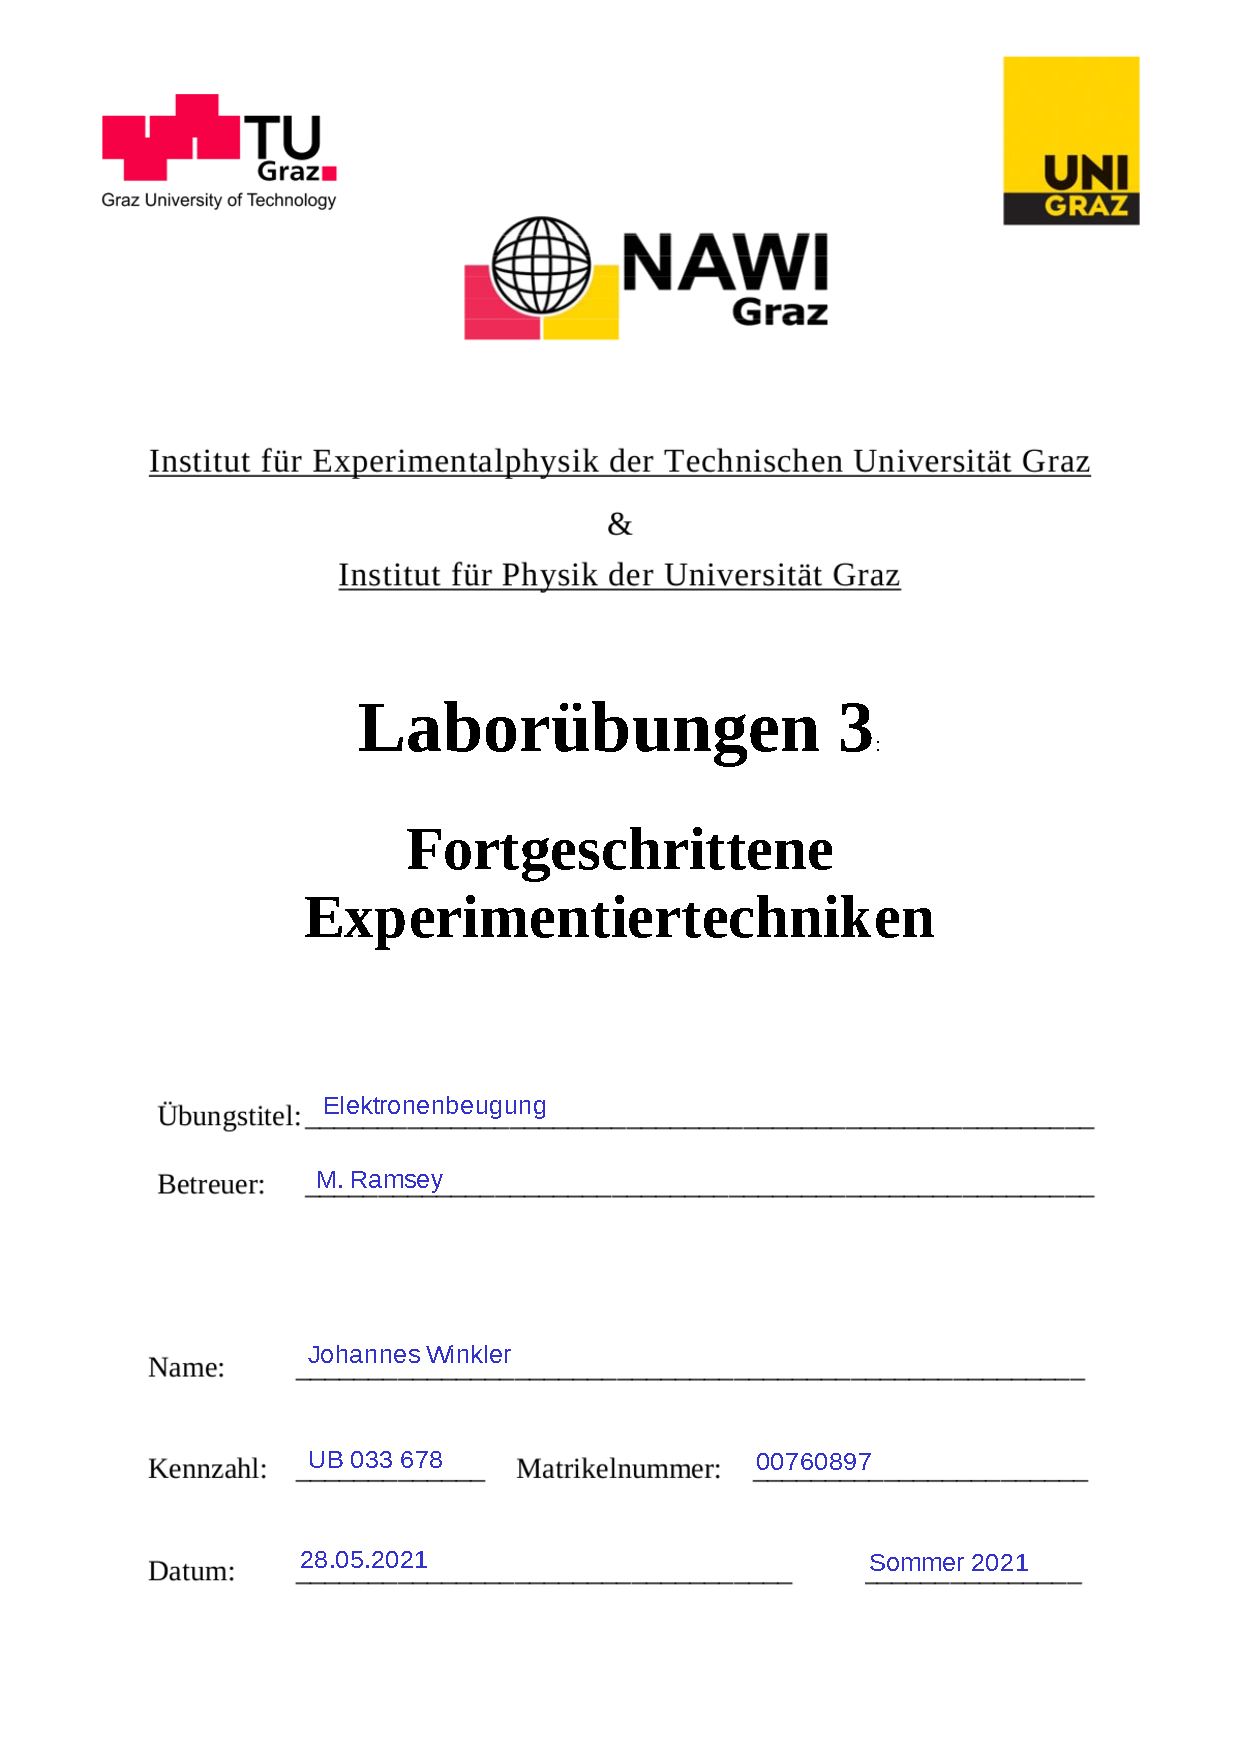
\includepdf{Deckblatt_neu_custom.pdf}

\tableofcontents
\newpage

\pagestyle{fancy}

\section{Aufgabenstellung}

\begin{enumerate}
\item Aufnahme und Kalibrierung eines Röntgenenergiespektrums
\item Bestimmen der $K_\alpha$-Energie
\item Ermittlung der Abschirmkonstante
\item Analyse einer unbekannten Probe
\end{enumerate}


%\begin{figure}[H]
%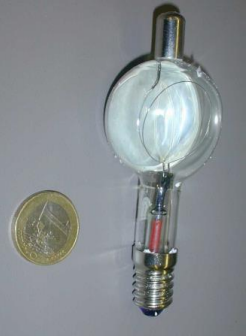
\includegraphics[scale=1.4]{versuch3.png}
%\caption{Vakuum Photozelle. Quelle: \cite{moodle}}
%\end{figure}

\section{Grundlagen}

Durch Bestrahlung von Atomen mit hochenergetischer Röntgenstrahlung können Elektronen aus einer inneren Schale herausgeschlagen werden (Ionisierung). Die dadurch entstehenden Lücken werden von äußeren Elektronen gefüllt, die dadurch Energie verlieren, diese Energie wird als Röntgenstrahlung emittiert.

Es gibt einen Zusammenhang zwischen der Energie, der Schalen im Atommodell und der Kernladungszahl. Dieser Zusammenhang wird Moseley'sches Gesetz. Als Formel ist das Gesetz in einer für uns nützlichen Variante
\begin{align}
\sqrt{\frac{E}{R_y}} = (Z - \sigma_{2,1}) \cdot \sqrt{ \frac{1}{n_1^2} - \frac{1}{n_2^2}}
\label{eq:moseley}
\end{align}
mit der Rydberg-Konstanten $R_y = 13.605~$eV laut \cite{ry}.



\begin{figure}[H]
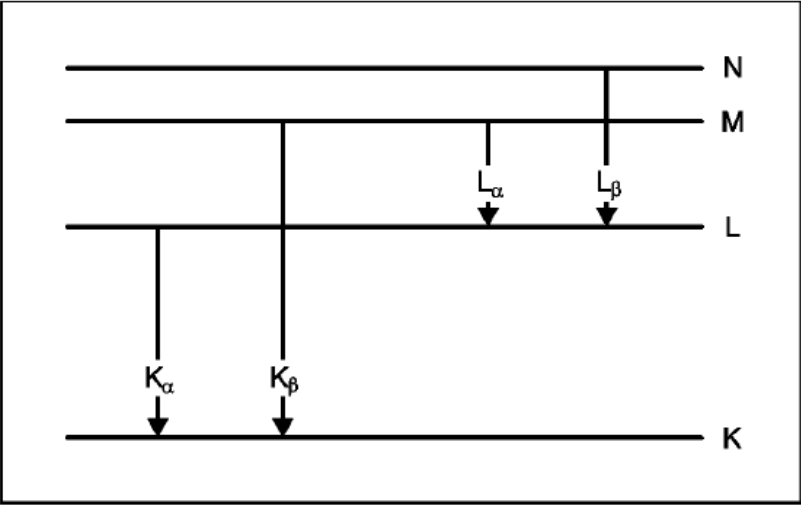
\includegraphics[scale=1.79]{moseley.png}
\caption{Einfache Darstellung der Röntgenlinien eines Atoms. Quelle: \cite{moodle}}
\label{fig:moseley}

\end{figure}


%\begin{figure}[H]
%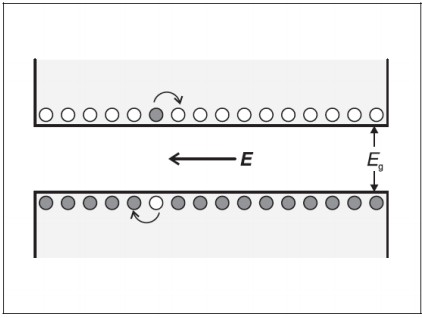
\includegraphics[scale=1.4]{bandabstand.png}
%\caption{Veranschaulichung des Bändermodells. Quelle: \cite{moodle}}
%\label{fig:bandabstand}
%\end{figure}



\section{Versuchsaufbau}

\begin{figure}[H]
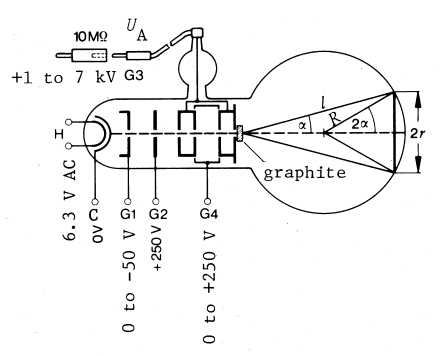
\includegraphics[scale=1.79]{versuchsaufbau.png}
\caption{Aufbau des Versuchs. Quelle: \cite{moodle}}
\label{fig:aufbau}

\end{figure}



\section{Geräteliste}


\begin{table}[H]
\caption{Liste der verwendeten Geräte}
~
\begin{tabular}{l|l}
 & Geräte  \\
\hline
1 & Röntgengerät, Leybold \\
2 & CASSY-Sensor \\	
3 & Metallplätchen aus diversen Materialien\\
4 & Computer mit CASSY-Lab2
\end{tabular}

\end{table}


\section{Durchführung und Messergebnisse}

Zuerst wurde das Röntgengerät eingeschalten und der Computer mit CASSY-Lab 2 gestartet. Für die Messung im CASSY-Lab2 wurden 512 Kanäle, negativer Puls ein Verstärkungsfaktor von -2.5 und eine Messdauer von 200~s eingestellt. Am Röntgengerät selbst wurde eine Spannung von 30~kV eingestellt mit einem Emissionsstrom von 1~mA. Danach wurde das Gerät gestartet und jeweils die Spektren von Eisen und Molybdän aufgenommen.

Die Spektren von Eisen und Molybdän zur Kalibrierung befinden sich in Grafik~\ref{fig:vor_kalibrierung_fe_mo}. In Grafik~\ref{fig:vor_kalibrierung_alle} sind alle bekannten Spektren nochmals in einer Grafik zusammengefasst. Zusätzlich liegt ein Spektrum einer unbekannten Probe vor. Dieses ist in Grafik~\ref{fig:vor_kalibrierung_alle_unbekannt}

\begin{figure}[H]
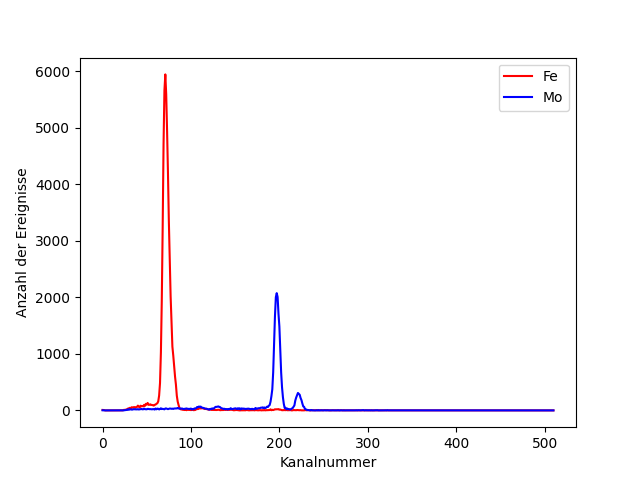
\includegraphics[scale=0.7]{vor_kalibrierung_fe_mo.png}
\caption{Spektrum der Elemente Eisen und Molybdän, die zur Kalibrierung verwendet werden.}
\label{fig:vor_kalibrierung_fe_mo}

\end{figure}


\begin{figure}[H]
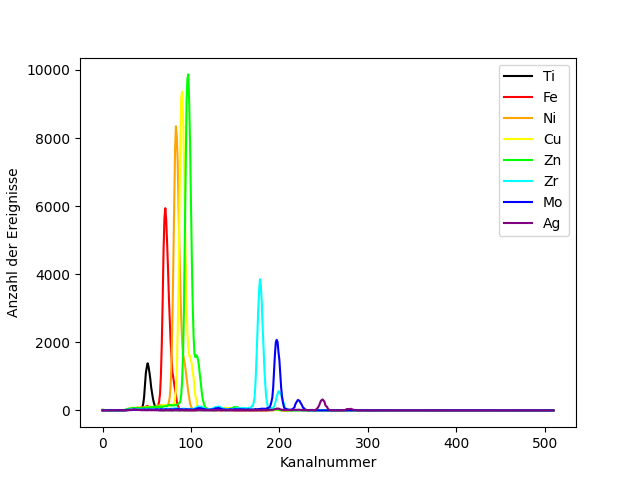
\includegraphics[scale=0.7]{vor_kalibrierung_alle.png}
\caption{Unkalibrierte Spektren aller bekannten Elemente.}
\label{fig:vor_kalibrierung_alle}

\end{figure}



\begin{figure}[H]
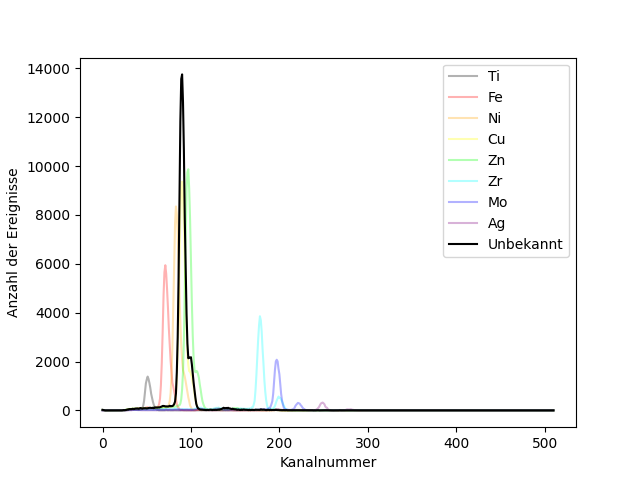
\includegraphics[scale=0.9]{vor_kalibrierung_alle_inkl_unbekannt.png}
\caption{Spektrum eines unbekannten Elementes, zum Vergleich die Spektren aus Grafik~\ref{fig:vor_kalibrierung_alle} im Hintergrund. Man kann hier schon eine deutliche Übereinstimmung mit Kupfer erkennen.}
\label{fig:vor_kalibrierung_alle_unbekannt}

\end{figure}

\section{Auswertung}

Zuerst muss das Röntgengerät kalibriert werden. Aus den Daten für Grafik~\ref{fig:vor_kalibrierung_fe_mo} zeigt sich, dass die Peaks für Eisen am Kanal 71 und für Molybdän am Kanal 197 liegen. Aus \cite{moodle} wissen wir die Energien für diese Elemente. Dadurch lassen sich die x-Werte linear transformieren. Die folgende Tabelle zeigt alle dafür notwendigen Werte

\begin{table}[H]
\caption{Lineare Transformation der Kanalnummer zu einer angegebenen Energie.}

\begin{tabular}{c|rr}
Element & Kanal / 1 & $E$ / keV \\
\hline
Eisen & 71 & 6.40 \\
Molybdän & 197 & 17.48 
\end{tabular}
\end{table}

Die lineare Transformation vom Kanal $x$ auf die dazugehörige Energie ist gegeben durch
\begin{align*}
\text{Energie} = 8.79\cdot 10^{-2}~\frac{\text{keV}}{\text{Kanal}}\cdot x + 0.16~\text{keV}
\end{align*}

Die folgende Tabelle beschreibt für alle Elemente jenen Kanal, wo der Peak (also die $K_\alpha$-Linie) ist. Der Kanal wurde dann anschließend in Energiewerte transformiert.

\begin{table}[H]
\caption{Peaks im Spektrum zum Finden der $K_\alpha$-Linie für jedes Material. Zusätzlich die Kernladungszahl für jedes Element. Zusätzlich wurde der Peak und die Energie für das unbekannte Material berechnet. Dieses stimmt eindeutig mit Kupfer überein.}
\label{tab:Energie}
\begin{tabular}{c|rrr}
Element & $Z$ & Kanal & $E$ / keV \\
\hline
Titan     & 22 &  51 &   4.64 \\
Eisen     & 26 &  71 &   6.40 \\
Nickel    & 28 &  83 &   7.46 \\
Kupfer    & 29 &  90 &   8.07 \\
Zink      & 30 &  97 &   8.69 \\
Zirkonium & 40 & 178 &  15.81 \\
Molybdän  & 42 & 197 &  17.48 \\
Silber    & 47 & 249 &  22.05 \\
\hline
unbekannt & -- & 90  &   8.07
\end{tabular}
\end{table}

Durch diese Transformation kann Grafik~\ref{fig:vor_kalibrierung_alle} nochmals mit korrekter Bezeichnung in der x-Achse dargestellt werden, siehe Grafik~\ref{fig:nach_kalibrierung_alle}. Durch Tabelle~\ref{tab:Energie} ist davon auszugehen, dass es sich bei der unbekannten Probe um Kupfer handelt. Grafik~\ref{fig:nach_kalibrierung_kupfer_unbekannt} stellt diese beiden Proben gegenüber.

\newpage

\begin{figure}[H]
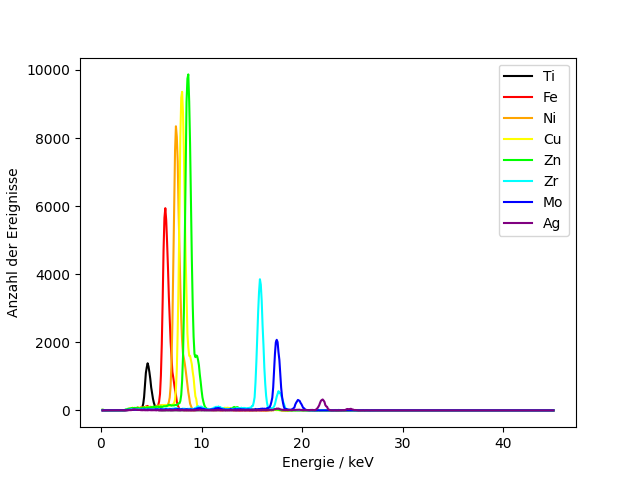
\includegraphics[scale=0.7]{nach_kalibrierung_alle.png}
\caption{Kalibrierte Spektren aller bekannten Elemente.}
\label{fig:nach_kalibrierung_alle}
\end{figure}
\begin{figure}[H]
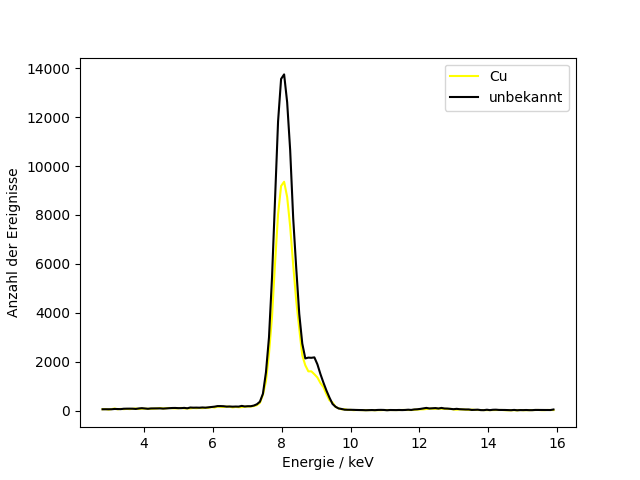
\includegraphics[scale=0.7]{nach_kalibrierung_kupfer_unbekannt.png}
\caption{Kalibrierte Spektren von Kupfer und der unbekannten Probe.}
\label{fig:nach_kalibrierung_kupfer_unbekannt}
\end{figure}

Nach dem Moseley-Gesetz aus Gleichung~\ref{eq:moseley} folgt für die Abschirmkonstante $\sigma_{2,1}$ durch Einsetzen von $n_1=1$ und $n_2=2$ und Umformung
\begin{align*}
Z - \sqrt{\frac{4\cdot E}{3\cdot R_y}} = \sigma_{2,1}
\end{align*}

Daraus kann für jedes Element die Abschirmkonstante $\sigma_{2,1}$ berechnet werden.


\begin{table}[H]
\caption{Berechnung der Abschirmkonstante $\sigma_{2,1}$ in Abhängigkeit von der Energie $E$.}

\begin{tabular}{c|rrrr}
Element & $Z$ &  $E$ / keV & $\sigma_{2,1}$  & $\Delta\sigma_{2,1}$ \\
\hline
Titan     & 22 &  4.64 & 0.673 & 0.026\\
Eisen     & 26 &  6.40 & 0.956 & 0.024\\
Nickel    & 28 &  7.46 & 0.970 & 0.023\\
Kupfer    & 29 &  8.07 & 0.877 & 0.021\\
Zink      & 30 &  8.69 & 0.824 & 0.021 \\
Zirkonium & 40 &  15.81 & 0.639  & 0.017 \\
Molybdän  & 42 &  17.48 & 0.611 & 0.013\\
Silber    & 47 &  22.05 & 0.512 & 0.012
\end{tabular}
\end{table}

Die Abschirmkonstante kann auch in Abhängigkeit von der Kernladungszahl grafisch dargestellt werden.

\begin{figure}[H]
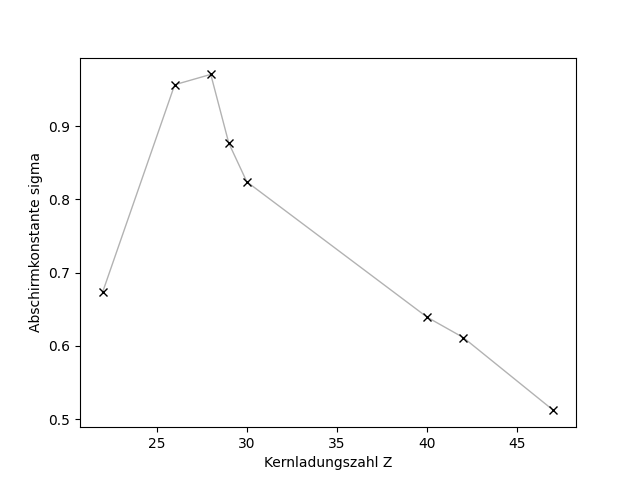
\includegraphics[scale=0.9]{abschirmkonstante.png}
\caption{Abschirmkonstante dargestellt in Abhängigkeit der Kernladungszahl.}
\label{fig:sigma}
\end{figure}





\section{Diskussion und Zusammenfassung}


Die Werte für die Energie bei den $K_\alpha$-Linien stimmen sehr gut mit der Literatur überein. Die $K_\beta$-Linien sind insbesondere für kleine Kernladungszahlen sehr schwer zu erkennen, da sie sehr dicht bei den $K_\alpha$-Linien liegen (man benötigt eine höhere Messauflösung um diese zu lokalisieren). Die Theorie lehrt uns aufgrund der Orbitalbesetzung, dass die Abschirmkonstante für Elemente mit Ordnungszahl < 28 steigt, und ab 30 wieder fällt. Die Messergebnisse entsprechen daher den theoretischen Erwartungen.


Das unbekannte Material dürfte Kupfer sein, da es sich gemäß Abbildung~\ref{fig:nach_kalibrierung_kupfer_unbekannt} sehr ähnlich zu Kupfer verhält. Es handelt sich tatsächlich um eine Kupfermünze, die hier vermessen worden ist.


\begin{thebibliography}{9}
\bibitem{moodle} G. Koller: Skript zu Röntgenfluoreszenz aus dem Moodle der Karl-Franzens Universität, Institut für Physik, 04.06.2021.
\bibitem{messmethoden}  R. Dämon: Einführung in die physikalischen Messmethoden, Graz 2016.
\bibitem{AKT}  J. Winkler: Unterlagen (Mitschrift) zur Atom-, Kern und Teilchenphysik Vorlesung des Wintersemesters 2020, Vorlesung gehalten von M. Schultze, Graz 2020.
\bibitem{demtroeder} W. Demtröder: \emph{Experimentalphysik 2 - Elektrizität  und Optik}, 7. Auflage, 2017.
\bibitem{python} Python-Skript zur Berechnung der Daten, zur Visualisierung und zum Generieren von \LaTeX-Code für diesen Bericht.
\bibitem{ry} \url{https://en.wikipedia.org/wiki/Rydberg_constant}, 04.06.2021.
\end{thebibliography}


\newpage 
%\appendix
%\section{Python Skript}



\definecolor{commentgreen}{RGB}{2,112,10}
\definecolor{eminence}{RGB}{108,48,130}
\definecolor{weborange}{RGB}{255,165,0}
\definecolor{frenchplum}{RGB}{129,20,83}

\lstdefinelanguage{python}{
    morekeywords={def, for, range, abs, return},
    otherkeywords={<-,->, |>, \%\{, \}, \{, \, (, )},
    sensitive=true,
    morecomment=[l]{\#},
    morecomment=[n]{/*}{*/},
    morecomment=[s][\color{purple}]{:}{\ },
    morestring=[s][\color{orange}]"",
    commentstyle=\color{commentgreen},
    keywordstyle=\color{eminence},
    stringstyle=\color{red},
	basicstyle=\ttfamily,
	breaklines,
	showstringspaces=false,
	frame=tb
}
%\lstinputlisting[language=Python,captionpos=b, label=lst:test,caption={Auswertung}]{script.py}

%\lstinputlisting[language=Python,captionpos=b, label=lst:test,caption={Bessel Auswertung}]{generate_numbers_bessel.py}



\end{document}